% ---------------------------------------------------------------------------
% PX915 individual project report -- Tristan McCarthy
% Build:  latexmk -pdf report.tex        (REVTeX 4-2 + natbib, refs.bib)
% ---------------------------------------------------------------------------
\documentclass[aps,prb,twocolumn,superscriptaddress,floatfix,nofootinbib]{revtex4-2}

\usepackage{graphicx}
\usepackage{amsmath,amssymb}
\usepackage{booktabs}
\usepackage[dvipsnames]{xcolor}
\usepackage[colorlinks=true,allcolors=blue!60!black]{hyperref}
\usepackage{siunitx}

\begin{document}

\title{Three-dimensional atom localisation with calibrated uncertainty from multislice
electron ptychography: mapping polar order in a PbTiO$_3$/SrTiO$_3$ superlattice}

\author{Tristan McCarthy}
\affiliation{HetSys Centre for Doctoral Training, University of Warwick, Coventry CV4 7AL, UK}
\author{Peng Wang}
\affiliation{Department of Physics, University of Warwick, Coventry CV4 7AL, UK}
\author{Nicholas D. M. Hine}
\affiliation{Department of Physics, University of Warwick, Coventry CV4 7AL, UK}

\date{\today}

\begin{abstract}
Polar vortices in ferroelectric superlattices are intrinsically three-dimensional: the
polarisation rotates along the electron beam as well as across it, so a projection image
integrates away the very structure it is used to measure. Multislice electron ptychography
(MEP) recovers depth from a single orientation, but converting its phase volume into atomic
coordinates is obstructed by an extremely anisotropic response --- $0.1$\,\AA{} in-plane
against $1$--$2$\,\AA{} along the beam --- which buries the oxygen sublattice under its
titanium neighbours. We simulate 4D-STEM of a relaxed PbTiO$_3$/SrTiO$_3$ supercell, invert it
by MEP, and localise every atom by fitting the volume as a superposition of a \emph{measured}
single-atom response. Against the known structure the method recovers $95.5\%$ of bulk oxygen
with $1.1\%$ species confusion, where the established route --- three-dimensional
deconvolution followed by peak detection --- reaches at most $59\%$; the entire advantage lies
in the axially overlapped oxygen (recall $82\%$ against $9$--$26\%$). Per-atom uncertainties
combine a \emph{joint} Cram\'er--Rao bound, which corrects the twofold variance inflation that
a per-peak bound misses at the $1.95$\,\AA{} Ti--O spacing, with distribution-free Mondrian
conformal calibration; the intervals hold their nominal coverage to within $1\%$, and the
procedure carries over with no retuning to an independent reconstruction at a different
sampling and dose. Propagating them
through the Ti--O$_6$ off-centring gives the local polarisation with error bars: the in-plane
component is recovered to a median $0.007$\,\AA{} and $0.9^\circ$, while the along-beam
component is not measured at all --- and the calibrated uncertainty reports this without
recourse to ground truth. First-principles core-hole DFT shows that the missing component is
nevertheless spectroscopically accessible: the O~K edge is $78\%$ dichroic with respect to the
polar-axis orientation, of which a monotonic $19\%$ is the ferroelectric displacement's own
signature, though recovering it requires a collection aperture $\lesssim2$\,mrad rather than
the $100$\,mrad ptychography optics.
\end{abstract}

\maketitle

% ===========================================================================
\section{Introduction}
% ===========================================================================

Ferroelectric oxide superlattices host polar textures --- vortices, skyrmions, labyrinths ---
that have no counterpart in bulk ferroelectrics and are now a mature field of their own
\citep{Yadav2016,Tang2015,Das2019,Junquera2023}. In PbTiO$_3$/SrTiO$_3$ (PTO/STO), competition
between elastic, electrostatic and gradient energies drives the local dipoles into
rotational arrangements whose topology, not merely whose magnitude, is the physical object of
interest. Establishing that topology experimentally means measuring a vector field at atomic
resolution, and the standard tool for doing so is atomic-resolution STEM: the polarisation is
inferred from the sub-\aa{}ngstr\"om offset of the B-site cation from the centre of its oxygen
cage, mapped column by column.

That measurement is a projection. A conventional STEM image integrates along the beam, so it
returns the component of the off-centring lying in the image plane and is blind to the
component along the viewing direction. For a uniformly polarised domain this is a minor
restriction, cured by imaging a second zone axis. For a vortex it is not: the polarisation
\emph{rotates with depth}, so different depths within a single atomic column carry different
--- sometimes opposing --- dipoles, and the projected image reports their average. The
structure that defines the texture is exactly the structure the measurement removes.

Multislice electron ptychography (MEP) offers a way out. By recording the full diffraction
pattern at every probe position and inverting a multislice forward model, MEP reconstructs the
specimen as a stack of slices rather than a single projection, achieving optical sectioning
from a \emph{single} orientation \citep{Gao2017,Chen2021,MaidenHumphryRodenburg2012}. Its
lateral resolution is set by the illumination angle rather than the lens
\citep{Nellist1995,Jiang2018,Nguyen2024}, and it has matured rapidly: dopant depths in bulk
crystals \citep{Chen2021}, oxygen vacancy sites in nickelates \citep{Dong2024}, sub-nanometre
depth resolution from a few coupled small-angle projections \citep{Dong2025}. The alternative,
atomic electron tomography, gives three-dimensional coordinates with quantified precision
\citep{Yang2017,Yang2021,Xu2015} but needs a large tilt series --- prohibitive for a
beam-sensitive oxide, and incompatible with the single-orientation acquisition a vortex
measurement must be built on.

The obstacle is what happens \emph{after} the reconstruction. A single-orientation measurement
is aperture-limited in depth: for convergence semi-angle $\alpha$ the lateral resolution scales
as $\lambda/2\alpha$ but the axial as $\lambda/\alpha^2$, which for the $300$\,keV,
$100$\,mrad probe used here are $\approx0.10$\,\AA{} and $\approx2.0$\,\AA{} respectively. The
reconstructed response of a single atom is therefore more than an order of magnitude longer
along the beam than across it. Since that length exceeds the $1.95$\,\AA{} Ti--O spacing of the perovskite
sublattice, neighbouring responses overlap: an oxygen atom sits inside the axial flank of its
titanium neighbour. Local peak detection cannot separate them, and the established remedy ---
three-dimensional Richardson--Lucy or maximum-entropy deconvolution of the volume followed by
peak analysis \citep{Ishizuka2021} --- was developed for sparse, isolated features rather than
for a dense sublattice. Meanwhile the two-dimensional community long ago settled on
model-based least-squares fitting of a peak superposition, whose defining virtue is that it
handles overlap explicitly \citep{DeBacker2016}. That machinery has not been carried into three
dimensions for every atom of a dense lattice at once.

There is a second gap, and for a physical conclusion it is the more serious one. A polarisation
map derived from located atoms is a difference of coordinates, each carrying an error; whether
a measured off-centring is real or is an artefact of localisation noise cannot be judged without
a per-atom uncertainty that is \emph{calibrated}, not merely reported. Reconstruction pipelines
rarely provide one. A least-squares covariance is optimistic on near-noiseless simulated data,
where the error is systematic rather than statistical, and the natural per-peak Cram\'er--Rao
bound is the bound with all neighbours known exactly --- precisely the assumption that fails on
an overlapped lattice.

This work addresses both gaps and applies the result to the physics. We (i) simulate 4D-STEM of
a relaxed PTO/STO supercell and reconstruct it by MEP; (ii) localise every atom by fitting the
phase volume as a superposition of a \emph{measured} single-atom response, extending
model-based quantification \citep{DeBacker2016} to three dimensions and to all species at once;
(iii) attach per-atom uncertainties that combine a joint Cram\'er--Rao bound with
distribution-free conformal calibration, and demonstrate that they transfer to an independent
reconstruction; (iv) propagate them into a Ti--O$_6$ polarisation map, showing quantitatively
which component of the polarisation the measurement does and does not determine; and (v) ask,
by core-hole DFT, whether the component ptychography misses is recoverable spectroscopically.
Throughout, the localisation never sees the ground truth: known coordinates are used only to
score the result.

% ===========================================================================
\section{Methods}
% ===========================================================================

\subsection{Model system}

The test object is a relaxed atomistic supercell of a PTO/STO superlattice provided by
collaborators --- $70.0\times70.0\times47.9$\,\AA{}, $19\,440$ atoms, $1944$ formula units of
each material. Both are perovskites (ABO$_3$): heavy Pb or Sr on the A site, Ti on the B site,
oxygen on an octahedral cage. In the PTO layers the B-site titanium and A-site lead displace
from their centrosymmetric positions, and the resulting dipoles order into the labyrinth
pattern characteristic of these superlattices. We quantify the local polarisation throughout
by the B-site off-centring
\begin{equation}
  \boldsymbol{\delta}_i \;=\; \mathbf{r}_{\mathrm{Ti},i} \;-\;
  \tfrac{1}{6}\!\!\sum_{j\in\mathrm{O}_6(i)}\!\!\mathbf{r}_{\mathrm{O},j},
  \label{eq:delta}
\end{equation}
the displacement of each titanium from the charge centre of its six nearest oxygens.
Figure~\ref{fig:sample}(a) maps its in-plane projection over the whole cell.

This is an exacting test on three counts: the scattering contrast spans two orders of magnitude,
from lead ($Z=82$) to oxygen ($Z=8$), so the light sublattice sits near the noise floor; the
signal is a sub-\aa{}ngstr\"om displacement of atoms $1.9$--$3.9$\,\AA{} apart; and the
polarisation varies along the beam as well as across it, twisting with depth into a vortex tube
within the scanned volume (Fig.~\ref{fig:sample}c). The beam is set along a pseudocubic
$\langle100\rangle$ direction, a $\approx70$\,\AA{} path; the known input coordinates are the
ground truth against which every result is scored.

\begin{figure*}[t]
  \centering
  
\includegraphics[width=0.76\linewidth]{figs/sample}\\[2pt]
  
\includegraphics[width=0.25\linewidth]{figs/tornado}
  \caption{The model system. (a) In-plane polarisation over the whole cell viewed down the beam,
    one mean-direction arrow per atomic column, resolving the polar domains and vortices. Shaded
    square: the $20$\,\AA{} scan window; shaded disc: the exit-wave footprint the recorded
    diffraction spans, which is why the full box is simulated. (b) Atomic columns in beam
    projection within the scan region with the overfocused probe ($\approx4$\,\AA) overlaid; the
    lead columns split into polar dumbbells. (c) The polarisation of the scanned volume in three
    dimensions: the local dipoles (arrows, coloured by depth) twist into a vortex tube along the
    beam --- the depth variation that a projection integrates away.}
  \label{fig:sample}
\end{figure*}

\subsection{4D-STEM simulation}

The simulation is the forward operator $\mathcal{S}$ mapping the structure to the data a
microscope would record, $\mathbf{I}=\mathcal{S}(\{\mathbf{r}_a,Z_a\})+\text{noise}$. A
convergent probe of semi-angle $\alpha=100$\,mrad at $300$\,keV ($\lambda=1.969$\,pm), focused
$20$\,\AA{} above the entrance surface, is propagated through the specimen by the multislice
recursion \citep{CowleyMoodie1957,Kirkland2010}
\begin{equation}
  \psi_{n+1} = \mathcal{P}_{\Delta z}\!\otimes\!\big[\,t_n(\mathbf{r})\,\psi_n(\mathbf{r})\,\big],
  \qquad t_n = \exp\!\big[\,i\,\sigma\, v_n(\mathbf{r})\,\big],
  \label{eq:multislice}
\end{equation}
with $v_n$ the projected potential of slice $n$, $\sigma$ the interaction constant and
$\mathcal{P}_{\Delta z}$ the Fresnel propagator; the recorded quantity is
$I(\mathbf{r}_p,\mathbf{k})=|\mathcal{F}\psi_N|^2$. We use abTEM \citep{MadsenSusi2021} on GPU
with Lobato potentials \citep{LobatoVanDyck2014}. Thermal motion enters in the frozen-phonon
approximation \citep{LoaneXuSilcox1991} as an incoherent average over $16$ configurations, with
displacement amplitudes set \emph{per species} from tabulated Debye--Waller factors
\citep{Peng1996}: lead and oxygen vibrate roughly twice as far as titanium ($B=0.90$ and $0.80$
against $0.45$\,\AA$^2$), so a single averaged amplitude would misweight the diffuse background
of exactly the species hardest to detect. A finite electron budget is imposed as shot noise,
$n \sim \mathrm{Poisson}(N_e\tilde I)$, over $D=10^{4}$--$10^{10}$\,e\,\AA$^{-2}$.

\subsection{Multislice ptychographic reconstruction}

Reconstruction inverts $\mathcal{S}$ by iterative ptychography
\citep{RodenburgFaulkner2004,Wakonig2020}. To resolve structure along the beam the single
multiplicative projection is replaced by a stack of $N_L$ transmission slices
\citep{MaidenHumphryRodenburg2012}; slices and probe are recovered jointly by minimising the
negative log-likelihood of the shot-noise model, implemented as the variance-stabilised
amplitude metric \citep{ThibaultGuizar2012} in the LSQ-ML engine of \citet{Odstrcil2018}
within PtychoShelves \citep{Wakonig2020}. Depth information is available because the
overfocused probe propagates dynamically through a specimen many times thicker than its depth
of focus and the reconstruction recovers that propagation slice by slice --- optical
sectioning, not tomography. We reconstruct $N_L=70$ slices (coherent,
$\Delta z_{\mathrm{rec}}\approx1.0$\,\AA) or $105$ (thermally averaged, $0.67$\,\AA).
Critically, \emph{no regularisation is applied to the inter-layer coupling}: the axial
structure is set by the data rather than by a smoothness prior, which would bias the very
coordinate we go on to quantify. For the dosed data the illumination is treated as a mixed
state \citep{ThibaultMenzel2013} with orthogonal probe relaxation \citep{Odstrcil2016}, so that
the thermal diffuse background is absorbed by incoherent degrees of freedom rather than forced
into the coherent object. All parameters are collected in Table~\ref{tab:params}.

\begin{table}[t]
  \centering \small
  \begin{tabular}{@{}lll@{}}
    \toprule
    Stage & Parameter & Value \\
    \midrule
    Sample & composition & PbTiO$_3$/SrTiO$_3$, $19\,440$ atoms \\
           & supercell & $70.0\times70.0\times47.9$\,\AA \\
    \addlinespace
    Probe  & energy / $\alpha$ & $300$\,keV / $100$\,mrad \\
           & defocus & $-20$\,\AA{} ($20$\,\AA{} overfocus) \\
    \addlinespace
    Scan   & window / step & $20$\,\AA{} / $0.10$--$0.15$\,\AA \\
    \addlinespace
    Sim.   & slice thickness & $2.0$\,\AA{} ($0.5$\,\AA{} fine) \\
           & frozen phonons & $16$ configs; per-species $B$ \\
           & detector & $200$\,mrad, binned to $356^2$\,px \\
           & dose & $10^{4}$--$10^{10}$\,e\,\AA$^{-2}$ (Poisson) \\
    \addlinespace
    Recon  & engine & PtychoShelves LSQ-ML \\
           & layers $N_L$ & $70$ / $105$ ($\Delta z_{\mathrm{rec}}=1.0$ / $0.67$\,\AA) \\
           & regularisation & inter-layer off; $\beta_{\mathrm{LSQ}}=0.1$ \\
    \addlinespace
    DFT    & code / functional & CASTEP \citep{Clark2005} / PBE \\
           & core hole & full ($1s^1$/$2p^5$), charge $+1$ \\
           & supercell & $2\times2\times2$ (40 atoms) \\
           & spectra & OptaDOS \citep{Morris2014}, $\hat{\mathbf{q}}$-resolved \\
    \bottomrule
  \end{tabular}
  \caption{Simulation, reconstruction and first-principles parameters.}
  \label{tab:params}
\end{table}

\subsection{Atom localisation}
\label{sec:atomfind}

\paragraph{Forward model.} We treat the reconstructed object as a sparse superposition of
identical single-atom responses,
\begin{equation}
  \phi(\mathbf{r}) = \sum_{i=1}^{N} \beta_i\, K(\mathbf{r}-\mathbf{r}_i) + b(\mathbf{r})
  + \varepsilon(\mathbf{r}), \qquad \beta_i \ge 0,
  \label{eq:forward}
\end{equation}
with $\phi$ the per-layer median-subtracted phase, $(\beta_i,\mathbf{r}_i)$ the amplitude and
three-dimensional position of atom $i$, and $b$ a slowly varying background removed by a
high-pass filter. The reconstruction is a nonlinear inverse problem, so
Eq.~\eqref{eq:forward} is an empirical linearisation rather than a derived identity; we test it
directly in Sec.~\ref{sec:res-fwd}.

The kernel $K$ is \emph{measured}, not parameterised: a single isolated atom is propagated
through the byte-identical simulation and reconstruction pipeline and its reconstructed
response is taken as $K$. This matters because $K$ is strongly anisotropic and its axial
profile is asymmetric, so no simple parametric form is faithful. We use the lead kernel for all
species --- an isolated oxygen or titanium does not reconstruct above the noise floor, so no
measured light-atom kernel exists --- on the argument that the response \emph{shape} belongs to
the imaging system while the amplitude $\beta$ carries $Z$.

\paragraph{Support selection.} With $K$ normalised to $\lVert K\rVert_2=1$, the least-squares
amplitude of a single source at $\mathbf{r}$ is the matched filter $(K\star R)(\mathbf{r})$
applied to the current residual $R$, and the position maximising it maximises the achievable
reduction in residual sum of squares. Selection is therefore greedy forward selection on the
dictionary $\{K(\cdot-\mathbf{r})\}$ --- matching pursuit \citep{MallatZhang1993}, equivalently
the CLEAN algorithm of radio astronomy \citep{Hogbom1974} --- with a minimum-separation
exclusion enforcing identifiability. Iteration stops when
$\max(K\star R) < k\,\sigma_{\mathrm{MF}}$, where $\sigma_{\mathrm{MF}}$ is a
median-absolute-deviation estimate of the matched-filter noise over the sub-median voxels of the
same subvolume and $k=2$ throughout. The threshold is noise-relative rather than absolute
because $(K\star R)$ scales with the phase amplitude of the reconstruction, which differs by a
factor of about two between the two reconstructions used here; an absolute threshold does not
transfer between them.

\paragraph{Refinement.} Writing $\theta_i=(\beta_i,\mathbf{r}_i)$, we minimise
$\lVert\phi-\sum_i\beta_iK(\cdot-\mathbf{r}_i)\rVert^2$ by block-coordinate descent: each atom
is updated in turn by Gauss--Newton steps on the local residual \emph{with the current models of
all other atoms subtracted}, so overlap between neighbours is accounted for to first order at
every update. Derivatives of $K$ are obtained by finite differences on the measured kernel. A
candidate is retained only if the normalised correlation between the local data (neighbours
removed) and its fitted response exceeds a fixed threshold --- a goodness-of-fit criterion on
\emph{shape}, independent of amplitude, so that weak but well-formed responses are not discarded
along with the poorly formed ones. This is model-based fitting of a peak superposition
\citep{DeBacker2016} carried into three dimensions with a measured rather than parametric
kernel; estimating depth by fitting the axial response is established for isolated dopants
\citep{Chen2021,Ishikawa2014}, and is applied here to every atom of a dense lattice.

\paragraph{Species and lattice-constrained detection.} Columns are typed from their own
fitted-amplitude statistics, which are well separated in this material; within mixed B--O
columns the two sublattices are separated by amplitude, with ambiguous cases resolved by
consistency with the local periodicity of already-assigned neighbours. Sites predicted by that
periodicity --- from the fitted atoms of the same column, never from the reference structure ---
but left empty by selection are re-examined at a reduced detection threshold with bounded
positional and amplitude tolerances. This deliberately trades false negatives against false
positives for the weakest species only; such detections are flagged in all outputs so that the
constrained and unconstrained populations can be reported separately, and every number below is
given for both.

\subsection{Uncertainty quantification}
\label{sec:uq}

We separate a \emph{model} standard error, computed without ground truth, from a
\emph{calibration} step that converts it into intervals with a stated coverage.

The model error has two terms, $\sigma^2=\sigma^2_{\mathrm{stat}}+\sigma^2_{\mathrm{sys}}$. The
statistical term is the Cram\'er--Rao bound of the \emph{joint} estimation problem: for the
stacked parameter vector $\theta=(\theta_1,\dots,\theta_N)$ the Fisher information of
Eq.~\eqref{eq:forward} under homoscedastic residuals is
$\mathbf{F}=\mathbf{J}^{\!\top}\mathbf{J}/s^2$, and the attainable variance of $\theta_i$ is the
corresponding diagonal block of $\mathbf{F}^{-1}$, \emph{not} the inverse of the diagonal block
$\mathbf{F}_{ii}$. The two coincide only for an orthogonal design; in general
$[\mathbf{F}^{-1}]_{ii}\ge[\mathbf{F}_{ii}]^{-1}$ and the ratio is the variance inflation factor
(VIF) of the overlapping templates. Evaluating $[\mathbf{F}_{ii}]^{-1}$ --- each atom fitted with
its neighbours held fixed --- is the per-peak bound used to predict single-column and
single-dopant precision \citep{DeBacker2016,Chen2021}; on a dense sublattice it is the bound
with all neighbours known exactly, and it is optimistic. We therefore assemble $\mathbf{J}$
over all atoms in a subvolume and invert $\mathbf{F}$ once (a $4N\times4N$ system with
$N\le45$), taking each atom's marginal variance. The systematic term $\sigma_{\mathrm{sys}}$ is
the position spread induced by kernel mismatch, estimated by fitting a synthetic response
generated with one measured kernel using another admissible kernel; it requires no ground truth
and so transfers to experimental data.

Intervals then follow by split-conformal calibration \citep{Vovk2005,AngelopoulosBates2023}: on
a volume with known positions we form nonconformity scores $s=|\Delta|/\sigma$ per axis and take
the empirical $(1-\alpha)$ quantile with the finite-sample correction, reporting
$q_{1-\alpha}\sigma$ as the half-width. This attains the target coverage by construction with no
Gaussian assumption. Because the error is strongly heteroscedastic across the lattice we
calibrate in the Mondrian (label-conditional) variant \citep{Vovk2003}, stratifying by species,
detection mode (unconstrained versus lattice-constrained) and depth band, so that coverage holds
\emph{per stratum} rather than only on average. The $95\%$ interval is the default in released
coordinates; the calibration table and per-stratum coverage are exported with the data, so a
dataset on which the calibration fails to transfer is identified rather than silently trusted.

\subsection{Polarisation from located atoms}

Equation~\eqref{eq:delta} is evaluated on the located atoms exactly as on the model: for each
located titanium, the six nearest located oxygens within $2.8$\,\AA{} form the cage, and
$\boldsymbol{\delta}$ is the offset of the titanium from their centroid. Titanium whose cage is
incomplete in the reconstruction is excluded and reported separately rather than completed from
the lattice. Uncertainty on $\boldsymbol{\delta}$ is propagated by Monte Carlo ($400$ draws)
from the per-atom conformal half-widths of Sec.~\ref{sec:uq} --- that is, from quantities
available \emph{without} ground truth, which is what a downstream user actually holds.

\subsection{First-principles EELS}
\label{sec:eels-method}

In core-loss EELS the beam electron ionises a core state; the energy-loss near-edge structure
(ELNES) is governed by the dynamic form factor entering the double-differential cross-section
\citep{Egerton2011}. For the small momentum transfer $\mathbf{q}$ of a near-axis collection the
dipole expansion gives
\begin{equation}
  S(\mathbf{q},E) \propto q^2 \sum_f
  \big|\langle f| \hat{\mathbf{q}}\cdot\mathbf{r}|i\rangle\big|^2\,\delta(E-E_f+E_i),
  \label{eq:dipole}
\end{equation}
so the ELNES measures the symmetry-projected unoccupied local density of states resolved along
$\hat{\mathbf{q}}$, which for a small on-axis aperture is essentially the beam direction. In an
anisotropic crystal this depends on the orientation of $\hat{\mathbf{q}}$ relative to the
lattice \citep{Nelhiebel1999} --- here, relative to the polar axis. Two consequences frame the
study. First, because $|\langle f|\hat{\mathbf{q}}\cdot\mathbf{r}|i\rangle|^2$ is even in
$\mathbf{q}$, the dipole ELNES sees the \emph{magnitude} of the along-beam polarisation but not
its \emph{sign}. Second, a real measurement integrates over the convergence and collection
apertures, and the anisotropic term is weighted by a geometric factor vanishing at the
\emph{magic angle} $\beta^\star\approx4\theta_E$, with $\theta_E=E/(\gamma m_0v^2)$
\citep{Jouffrey2004}.

We evaluate Eq.~\eqref{eq:dipole} with the plane-wave pseudopotential code CASTEP
\citep{Clark2005} using the core-hole method \citep{Gao2008}: the ionised atom carries an
on-the-fly-generated pseudopotential with one fewer core electron (a full core hole) plus a
neutralising background, in a $2\times2\times2$ supercell that dilutes the hole from its
periodic images, so the conduction states are computed in its presence. The core-to-conduction
matrix elements are contracted by OptaDOS \citep{Morris2014,Nicholls2012} into the core-loss
spectrum with $\hat{\mathbf{q}}$ set explicitly. The central quantity is the ELNES dichroism
\begin{equation}
  \Delta(E) = S(\mathbf{q}\!\parallel\!c,E) - S(\mathbf{q}\!\perp\!c,E),
  \label{eq:dichroism}
\end{equation}
the difference between probing along and across the polar axis, which by reciprocity is the
change in the measured edge when the polarisation rotates from along the beam to in-plane. We
take the O~K edge as the primary observable --- well described at the single-particle level and
an established probe of ferroelectric off-centring \citep{TorresPardo2011,Bugnet2016} --- and
treat Ti~L$_{2,3}$ for anisotropy trends only, since its $2p$ spin--orbit multiplet structure is
not captured by single-particle DFT \citep{Mizoguchi2009}. Calculations run on the Warwick
Blythe cluster; each PbTiO$_3$ core-hole SCF takes $40$--$45$\,min on $32$ cores and each
OptaDOS core-loss pass $75$--$90$\,min.

% ===========================================================================
\section{Results and discussion}
% ===========================================================================

\subsection{The measured response and the forward model}
\label{sec:res-fwd}

The reconstructed single-atom response (Fig.~\ref{fig:method}a) has full width at half maximum
$0.10$\,\AA{} in-plane against $1.0$\,\AA{} along the beam for the coherent reconstruction
and $2.0$\,\AA{} for the thermally averaged one --- the anisotropy the single-orientation
aperture scaling predicts, with the coherent figure a little sharper than the
$\delta z\approx\lambda/\alpha^2$ estimate on noiseless data. Because that
axial width is comparable to or larger than the $1.95$\,\AA{} Ti--O spacing, neighbouring
responses overlap and the design is not separable.

The decisive question is whether the apparent axial blur is \emph{overlap of a fixed response}
or a genuine loss of information. We test Eq.~\eqref{eq:forward} directly by fixing
$\{\mathbf{r}_i\}$ at the known positions and solving for $\{\beta_i\}$ only. A comb of measured
kernels at the true depths reproduces the observed depth profile of a mixed B--O column at a
median $r=0.94$ over $20$ columns (Fig.~\ref{fig:method}b), and $r=0.92$ in the full
depth--$x$ cross-section. The blur is therefore kernel overlap, not lost information --- which
is why a method that models the overlap can beat one that does not.

\begin{figure*}[t]
  \centering
  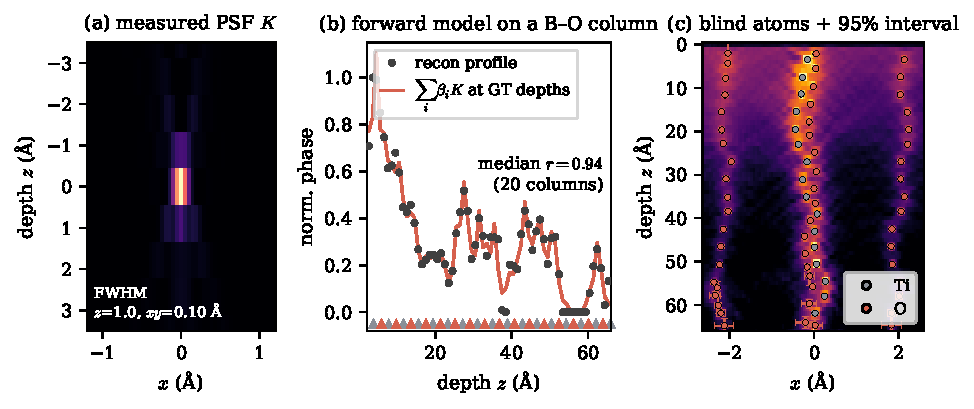
\includegraphics[width=\linewidth]{figs/fig_method}
  \caption{Model-based localisation. (a) The measured point-spread function $K$ (depth--$x$
    slice): tight in-plane, elongated along the beam by the aperture-limited axial resolution of
    a single-orientation measurement. (b) Direct test of the forward model,
    Eq.~\eqref{eq:forward}: the measured depth profile of a mixed Ti--O column against the
    superposition $\sum_i\beta_iK$ of the measured response at the \emph{known} atomic depths,
    matching at a median $r=0.94$ over $20$ columns. Triangles mark the true Ti (grey) and O
    (red) depths. The apparent $2$--$4$\,\AA{} axial blur is overlap of a fixed response, not a
    loss of information. (c) Blind atoms located on a raw cross-section, coloured by assigned
    species, with calibrated $95\%$ intervals.}
  \label{fig:method}
\end{figure*}

\subsection{Localisation performance}

Table~\ref{tab:detect} scores the method against the known structure, alongside the established
alternatives run on the \emph{same} volume with the \emph{same} measured kernel, each at its own
best-effort threshold. Over the bulk ($z=10$--$56$\,\AA, excluding the entrance and exit
artefact bands) the model fit recovers $95.5\%$ of oxygen, $96.4\%$ of titanium and $95.6\%$ of
lead, with $1.1\%$ of species labels wrong, in-plane RMS accuracy $0.032$\,\AA{} and depth RMS
$0.37$\,\AA.

The aggregate oxygen numbers understate what is actually being tested, so we split the oxygen
sublattice by its geometry. Oxygen that is \emph{in-plane isolated} --- sitting in its own
column, resolved laterally --- is found by every method, including raw peak-picking, at
$79$--$92\%$. Oxygen that is \emph{axially overlapped} --- sharing a column with titanium
$1.95$\,\AA{} away, hidden inside the flank of its neighbour's response --- is the hard case,
and it is where the methods separate completely: $82\%$ for the model fit against $26\%$ for
raw peak-picking, $13\%$ for maximum-entropy deconvolution and $9\%$ for Richardson--Lucy.
This is the entire advantage of the approach, and it is exactly the population that a
projection-blind, overlap-limited measurement must recover if the oxygen cage is to be
reconstructed at all.

\begin{table}[t]
  \centering \small
  \begin{tabular}{@{}lccccc@{}}
    \toprule
    & \multicolumn{3}{c}{recall (\%)} & \multicolumn{2}{c}{oxygen split (\%)} \\
    \cmidrule(lr){2-4}\cmidrule(lr){5-6}
    method & Pb & Ti & O & isolated & \textbf{overlapped} \\
    \midrule
    3-D peak-pick, raw            & 93 & 88 & 72 & 91 & 26 \\
    RL deconv.\ $+$ peak-pick     & 93 & 87 & 58 & 79 & \phantom{0}9 \\
    MEM deconv.\ $+$ peak-pick    & 93 & 89 & 59 & 79 & 13 \\
    1-D per-column deconv.        & 91 & 65 & 49 & 62 & 20 \\
    \textbf{3-D model fit}        & 88 & 89 & \textbf{89} & 92 & \textbf{82} \\
    \quad unconstrained only      & 88 & 89 & 86 & 92 & 71 \\
    \quad bulk, $z=10$--$56$\,\AA & \textbf{96} & \textbf{96} & \textbf{96} & --- & --- \\
    \bottomrule
  \end{tabular}
  \caption{Recovery of each sublattice, whole field unless stated, on the same reconstruction
    with the same measured kernel. ``Isolated'' oxygen occupies its own column; ``overlapped''
    oxygen shares a column with titanium $1.95$\,\AA{} away. Precision is $0.97$ for the model
    fit ($0.98$ unconstrained) against $0.84$--$0.99$ for the baselines; only the model fit
    returns species labels and per-atom uncertainties.}
  \label{tab:detect}
\end{table}

Two negative results deserve emphasis because they run against expectation.
First, \textbf{deconvolution before detection does not help, and Richardson--Lucy actively
hurts the oxygen}: both restoration routines \emph{lose} oxygen relative to peak-picking the
raw volume ($58$--$59\%$ against $72\%$). They redistribute dynamic range towards the strongly
scattering species, so weak oxygen falls below any relative floor, and they cannot restore the
axial spatial frequencies a single-orientation measurement never records --- the frequencies
that separate an oxygen atom from the flank of its titanium neighbour. Ishizuka \emph{et al.}
report maximum entropy as the stronger routine \citep{Ishizuka2021}; we reproduce no meaningful
advantage on a \emph{dense} lattice, consistent with that literature's own scope of sparse
dopants and adatoms. The limit is structural, not a tuning artefact.
Second, \textbf{on noiseless data a good peak-picker is competitive on the heavy atoms}. We
report this rather than a flattering weaker baseline: with no shot noise a raw local maximum is
already a clean estimator of an isolated bright column, so the margin quoted here is a lower
bound on the method's advantage, and the discriminating comparison is at finite dose
(Sec.~\ref{sec:dose}). What a peak-picker cannot provide at any dose is a species label or a
calibrated error bar.


\subsection{Calibrated uncertainty}

Figure~\ref{fig:uq}(a) quantifies why a per-peak bound is inadequate here. The variance
inflation factor of the joint fit is $1.04$ at the $3.9$\,\AA{} heavy-atom spacing --- where
atoms are effectively independent --- but $2.02$ in depth (and $2.28$ in amplitude) at the
$1.95$\,\AA{} Ti--O spacing, so a per-peak Cram\'er--Rao bound understates $\sigma_z$ by
$\approx1.4\times$ for every apical oxygen. Since $85\%$ of atoms in the field have a neighbour
within $2.5$\,\AA, the per-peak form is optimistic almost everywhere. Inverting the full Fisher
matrix restores the inflation per atom automatically, with no tuned constant.

Even so, the raw model $\sigma$ treated as Gaussian is badly miscalibrated on near-noiseless
simulation, covering only $\approx8\%$ of atoms at a nominal $68\%$ (Fig.~\ref{fig:uq}b): with
no shot noise the residual-based variance is near zero while the true error is dominated by
systematics the residual cannot see. Conformal calibration supplies the missing scale
empirically. Held out on a $50/50$ split, the conformal interval tracks the ideal diagonal
across the whole range of nominal coverage, reaching $69/69/69\%$ in $(x,y,z)$ at a $68\%$
target and $96/96/96\%$ at $95\%$. The Mondrian stratification is not cosmetic: the per-stratum
quantiles $q_{68}(z)$ range from $6.7$ to $14.4$, a factor of $2.2$, so a single pooled constant
necessarily leaves some strata conservative and others optimistic --- visible in
Fig.~\ref{fig:uq}(c), where pooling drops the worst stratum to $84\%$ against a $95\%$ target
while the label-conditional quantile restores every stratum to $95$--$100\%$.

\begin{figure*}[t]
  \centering
  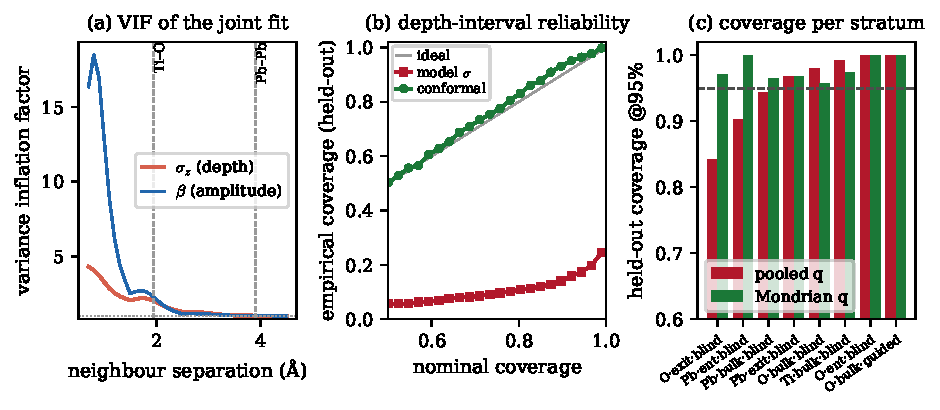
\includegraphics[width=\linewidth]{figs/fig_uncertainty}
  \caption{Calibrated uncertainty. (a) Variance inflation factor of the joint fit against
    neighbour separation: near unity at the $3.9$\,\AA{} heavy-atom spacing but ${\approx}2$ in
    depth (and larger in amplitude) at the $1.95$\,\AA{} Ti--O spacing, so a per-peak
    Cram\'er--Rao bound is optimistic wherever responses overlap. (b) Held-out reliability of
    the depth interval: the raw model standard error treated as Gaussian (red) severely
    under-covers on near-noiseless data, while the conformal interval (green) tracks the ideal
    diagonal. (c) Held-out coverage at the $95\%$ level for the strata where a single pooled
    quantile (red) departs most from target; the label-conditional quantile (green) restores
    coverage in each. Split-conformal, $50/50$ calibration/test split.}
  \label{fig:uq}
\end{figure*}

The decisive test of an uncertainty estimate is whether it survives a change of dataset. We
applied the identical code, with no tuned constants, to an independent reconstruction of the
same material at a different in-plane sampling ($0.10$ against $0.15$\,\AA), a different slice
discretisation ($105$ against $70$ layers), roughly half the phase amplitude and real
reconstruction noise. Re-running the conformal step on that volume's own atoms gives
$69/69/69\%$ at the $68\%$ target and $96/96/96\%$ at $95\%$ --- coverage as good as on the
volume the method was developed on. For comparison, the hand-tuned per-species error floors used
in an earlier version of this work, calibrated to $68\%$ coverage on the first volume,
transferred to $38/47/56\%$ on the second. The per-stratum quantiles on the harder volume span
an even wider range ($10.9$ to $23.3$), which is exactly the regime a single floor cannot serve
and conformal handles for free.

Three limitations should be stated plainly. The interval is a \emph{localisation} interval,
conditional on the atom having been correctly detected and typed; a spurious detection or a
species swap is a different failure mode, reported separately as precision ($0.97$) and
confusion ($1.1\%$). The species posterior we export is a within-column amplitude confidence and
is not itself calibrated, though it concentrates the residual errors usefully: labels below
$0.9$ are enriched for mislabelling by more than an order of magnitude over the base rate.
And conformal calibration assumes exchangeability between calibration and test atoms, which is
why the workflow re-runs the calibration per volume and exports the per-stratum coverage so
that a failure is visible.

\subsection{Behaviour at finite dose}
\label{sec:dose}

Table~\ref{tab:dose} runs the same configuration over a dose series on the independent
reconstruction. Performance is maintained to $10^{8}$\,e\,\AA$^{-2}$ and collapses below
$10^{6}$. The residual gap to the coherent reference (Ti $74\%$ against $89\%$) is not
attributable to the localisation constants but to a genuinely harder reconstruction: a
$2.0$\,\AA{} axial kernel against $1.0$\,\AA, and depth-registration correlation $0.44$
against $0.63$.

Two lessons generalise. First, \textbf{precision is not a safety indicator}. At
$10^{6}$\,e\,\AA$^{-2}$ precision reads $0.95$ --- apparently healthy --- while titanium recall
is $25\%$, oxygen $7\%$ and $38\%$ of species labels are wrong: the surviving bright lead atoms
are correctly placed, and precision measures only them. Species confusion and $\sigma$-coverage
are the diagnostics that fire, and the released pipeline prints both as health warnings.
Second, \textbf{species assignment is coupled to depth registration}. A $1$\,\AA{} depth error
on a lattice whose Ti and O alternate every $1.95$\,\AA{} swaps labels wholesale; correcting the
depth offset from $1.26$ to $0.29$\,\AA{} took titanium recall from $53\%$ to $74\%$ and
confusion from $19.0\%$ to $13.7\%$ at $10^{10}$\,e\,\AA$^{-2}$. Sub-\aa{}ngstr\"om depth
accuracy is not merely a precision figure; it is a prerequisite for correct chemistry.

\begin{table}[t]
  \centering \small
  \begin{tabular}{@{}lccccc@{}}
    \toprule
    dose (e\,\AA$^{-2}$) & precision & Pb & Ti & O & confusion \\
    \midrule
    $10^{10}$ & 0.83 & 86\,\% & 74\,\% & 63\,\% & 13.7\,\% \\
    $10^{8}$  & 0.87 & 87\,\% & 72\,\% & 67\,\% & 11.8\,\% \\
    $10^{6}$  & 0.95 & 75\,\% & 25\,\% & \phantom{0}7\,\% & 38.0\,\% \\
    $10^{4}$  & ---  & \phantom{0}0\,\% & \phantom{0}0\,\% & \phantom{0}0\,\% & --- \\
    \bottomrule
  \end{tabular}
  \caption{Dose series on an independent reconstruction ($105$ layers, $0.10$\,\AA{} sampling),
    run with the \emph{same} configuration as the coherent reference. The $10^{6}$ row is the
    case in point for precision being uninformative. A guided-detection deduplication guard
    added subsequently reduces the $10^{10}$ confusion to $12.4\%$ with titanium recall
    unchanged.}
  \label{tab:dose}
\end{table}

\subsection{Polarisation with error bars}
\label{sec:pol}

We now close the loop to the physical observable. Evaluating Eq.~\eqref{eq:delta} on the
located atoms, $72\%$ of bulk titanium acquire a complete oxygen cage from blindly located
oxygens alone; $171$ of these match a ground-truth titanium and are scored in
Fig.~\ref{fig:pol}.

The in-plane off-centring is recovered essentially exactly. The median error in
$\delta_x$ is $0.005$\,\AA{} and in $\delta_y$ $0.004$\,\AA{}, against a true in-plane
off-centring of mean magnitude $0.274$\,\AA; the recovered mean magnitude is $0.273$\,\AA. As a
vector the in-plane off-centring has median error $0.007$\,\AA{} and $90$th percentile
$0.017$\,\AA, and its \emph{direction} --- the quantity a vortex map is made of --- has median
error $0.9^\circ$, with $95\%$ of titanium within $30^\circ$. The correlation between recovered
and true $\delta_x$ is $0.96$ over all matched atoms and $1.00$ once a small tail is excluded.

That tail is the honest caveat. Five per cent of titanium have a cage of the wrong composition
--- a missing or misassigned oxygen displaces the centroid --- and for these the in-plane error
jumps to a median of $0.45$\,\AA, comparable to the signal itself. Crucially, the propagated
positional interval does \emph{not} cover them: it covers $99\%$ of the well-caged titanium but
only $12\%$ of the tail. This is not a failure of the calibration but a statement of its scope,
and it is the same caveat as in Sec.~\ref{sec:uq} propagated forward. The interval is
conditional on correct detection; a gross error in cage \emph{composition} is a detection
failure, and it must be reported through the detection metrics (precision, confusion, cage
completeness) rather than absorbed into a positional error bar. A practical map should therefore
carry both, and the $28\%$ of titanium with incomplete cages should be shown as absent rather
than interpolated.

The along-beam component tells the opposite story, and it is the more consequential result. Its
true spread across the scanned volume is small ($\sigma=0.074$\,\AA, since in this zone axis the
vortex polarisation is predominantly in-plane), while the propagated uncertainty on $\delta_z$
is $0.237$\,\AA{} --- more than three times the entire signal. The measured correlation with
truth is correspondingly poor ($r=0.42$, median error $0.122$\,\AA). \textbf{The along-beam
component of the polarisation is not measured by this experiment.} The value of the calibrated
uncertainty is that it says so \emph{blind}: comparing the propagated $\sigma_z$ with the spread
of the recovered $\delta_z$ requires no ground truth, and it correctly declares the along-beam
map uninformative while certifying the in-plane map to $0.01$\,\AA. Propagated intervals cover
$95/93/99\%$ of true errors in $(x,y,z)$ at a $95\%$ target, so the uncertainties are honest in
both directions --- neither the confidence in-plane nor the pessimism along the beam is
overstated.

This is a quantitative statement of the limitation that motivated the second half of the
project. Depth \emph{localisation} of individual atoms is good --- $0.37$\,\AA{} RMS, comfortably
better than the $\approx2$\,\AA{} depth resolution, in the same way that single-molecule
localisation beats the diffraction limit \citep{Thompson2002}. But a polarisation is a
\emph{difference} of two such coordinates, and differencing two $0.3$\,\AA{} depth errors
cannot resolve a $0.07$\,\AA{} displacement. In-plane the same argument runs the other way: the
in-plane error is $0.03$\,\AA{} against a $0.27$\,\AA{} signal, so the map is quantitative.

\begin{figure*}[t]
  \centering
  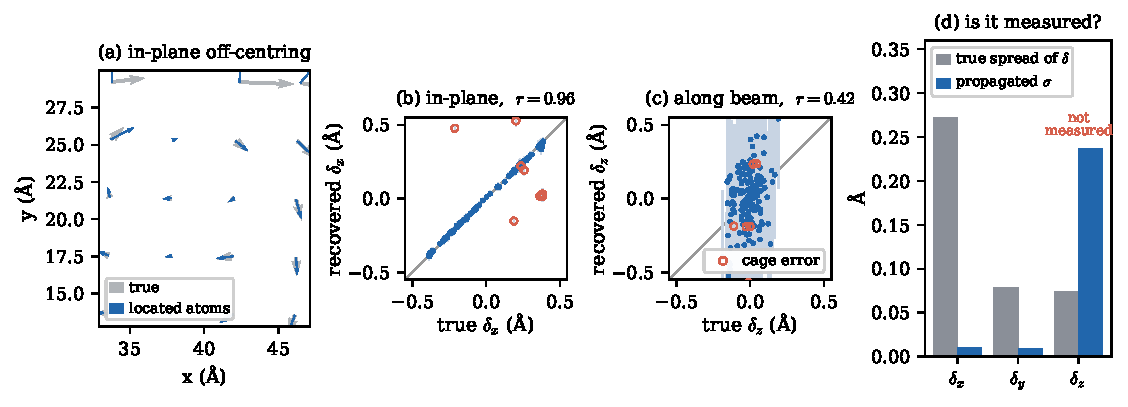
\includegraphics[width=\linewidth]{figs/fig_polarisation}
  \caption{Local polarisation from the located atoms. (a) In-plane Ti--O$_6$ off-centring
    averaged per atomic column: recovered (blue) over ground truth (grey). (b) Recovered against
    true in-plane off-centring, with propagated $95\%$ intervals; open red circles mark the
    $5\%$ of titanium whose oxygen cage has the wrong composition. (c) The same for the
    along-beam component. (d) The propagated uncertainty against the true spread of each
    component: in-plane the uncertainty is a small fraction of the signal, along the beam it
    exceeds it --- a ground-truth-free statement that the along-beam polarisation is not
    determined by this measurement.}
  \label{fig:pol}
\end{figure*}

\subsection{Can EELS see the missing component?}

The second phase asks whether the along-beam polarisation, invisible to a projected or
depth-differenced position measurement, leaves a spectroscopic fingerprint. The calculation was
built as a validated staircase, each step gated before the next.

\paragraph{Validation.} CASTEP/PBE reproduces the ferroelectric instability: single-point
energies across a displacement series $\mathbf{u}=s\,\mathbf{u}_0$ at fixed tetragonal strain
place the fully polar structure $203$\,meV per formula unit below the centrosymmetric reference,
monotonically, with the descent flattening towards $s=1$ so that the experimental displacement
sits at the PBE minimum. The core-hole recipe was then fixed by reproducing a known edge: the
rutile TiO$_2$ O~K ELNES comes out with its textbook shape, the t$_{2g}$/e$_g$ near-edge peaks
split by $2.7$\,eV (experiment $2.5$--$3$\,eV) with $e_g>t_{2g}$, followed by the broad
O~$2p$--Ti~$4sp$ band. As an artefact check, the dichroism of the \emph{cubic} cell computed at
the isotropic Ti site is $0.02\%$ --- the two spectra are identical, as symmetry demands, so any
dichroism elsewhere is physical rather than numerical.

\paragraph{The signal.} For the tetragonal cell with its polar axis along the beam, the O~K edge
is strongly dichroic: $\max|\Delta|/\max S = 78\%$ and $\int|\Delta|/\int S=47\%$
(Fig.~\ref{fig:eels}). The origin is a clean $\sigma/\pi$ anisotropy: with
$\mathbf{q}\perp c$ the edge shows a sharp $\pi^*$ peak at $\approx8.5$\,eV above onset from
O~$2p_{x,y}$, while with $\mathbf{q}\parallel c$ it shows $\sigma^*$ features at
$\approx11$ and $18.5$\,eV from the O~$2p_z$ pointing along the Ti--O--Ti chain. Orientation of
the polar axis relative to the beam therefore imprints strongly on the O~K edge, far above any
detectability floor.

\paragraph{Decomposition.} A large orientation dichroism is not by itself a polarisation
measurement, because the tetragonal \emph{backbone} is anisotropic even without off-centring.
Holding the lattice parameters fixed and varying only the internal displacement $s$ separates
the two (Fig.~\ref{fig:eels-scan}). At $s=0$ --- zero polarisation, full tetragonal strain ---
the dichroism is already $70.1\%$; at $s=1$ it is $78.2\%$. So roughly $70$ of the $78$ points
are the strain-induced backbone $\sigma/\pi$ anisotropy, and the ferroelectric off-centring's
own signature is the remaining, monotonic contribution: an $18.7\%$ change in the
along-beam-probed O~K spectrum between $s=0$ and $s=1$ ($4.3\%$ at $s=0.5$), plus $8$ points of
additional dichroism. This is the first-principles counterpart of the empirical observation that
the O~K edge responds to titanium off-centring \citep{Bugnet2016}, and it is what makes the
measurement a polarisation probe rather than merely a strain probe.

\paragraph{Detectability.} The intrinsic dichroism must then survive the acquisition geometry.
For the O~K edge at $300$\,keV, $\theta_E=1.09$\,mrad and the magic angle is $4.32$\,mrad
$=3.98\,\theta_E$, reproducing the textbook factor of $\approx4$ and validating our aperture
model. Folding the intrinsic anisotropy through the collection geometry gives a surviving
fraction of $0.62$ at $\beta=1$\,mrad, $0.28$ at $2$\,mrad, $-0.04$ at $5$\,mrad and
$-0.33$ at $100$\,mrad. The $100$\,mrad convergence of the ptychography probe therefore lies far
past the magic angle and averages the anisotropy away --- indeed inverts its sign. \emph{A
combined ptychography-plus-EELS experiment using one pixelated detector with a central hole
would collect at $\beta\approx100$\,mrad and wash out precisely the signal it was built to
measure.} Recovering the along-beam polarisation requires a dedicated small EELS aperture,
$\lesssim2$\,mrad; at a $2\%$ fractional anisotropy this needs $\approx4.5\times10^{4}$
counts per channel for SNR $3$, which sets the dose target.

\paragraph{Two intrinsic limits.} First, the dipole ELNES is even in $\mathbf{q}$, so it
measures the \emph{magnitude} of the along-beam polarisation but not its sign; distinguishing
$+P$ from $-P$ needs beyond-dipole or off-axis momentum transfer. A dynamical multislice
core-loss simulation of up- and down-polarised domains confirms this directly: the two give O~K
spectra identical to within $1.0\%$. Second, in the actual labyrinth viewed along this zone axis
the polarisation is mostly in-plane --- over $2560$ polar titanium, the median angle from the
beam is $82^\circ$ (interquartile range $73$--$87^\circ$), an along-beam fraction of only
$\approx0.14$. The full along-beam case computed here is therefore an upper bound for this
orientation; a different zone axis would raise the along-beam share, and the technique is best
suited to geometries chosen for it.

\begin{figure*}[t]
  \centering
  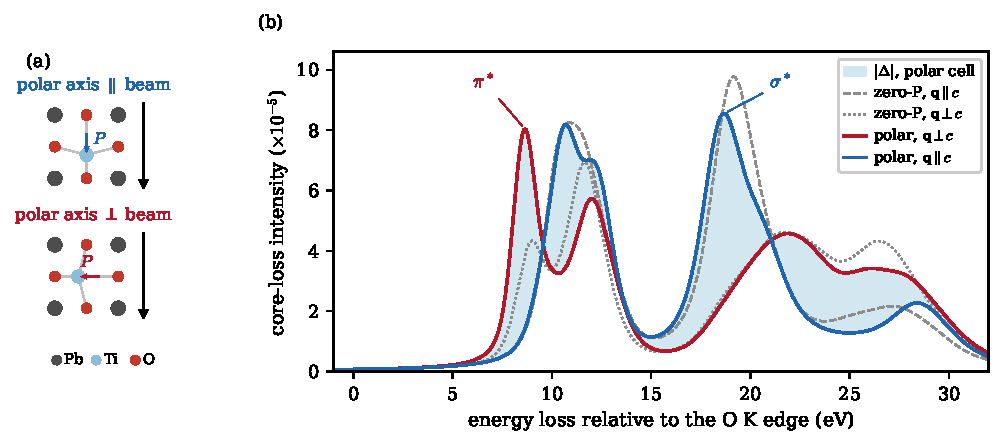
\includegraphics[width=0.82\linewidth]{figs/eels_dichroism}
  \caption{Orientation dichroism of the PbTiO$_3$ O~K edge from core-hole CASTEP $+$ OptaDOS.
    With the momentum transfer across the polar axis ($\mathbf{q}\perp c$, beam $\perp$
    $\mathbf{P}$) the edge shows a sharp $\pi^*$ peak; along it ($\mathbf{q}\parallel c$, beam
    $\parallel\mathbf{P}$) it shows the $\sigma^*$ features of the O~$2p_z$ states directed
    along the Ti--O--Ti chain. Grey curves are the same two orientations for the
    zero-polarisation (non-polar, equally strained) reference, isolating the backbone
    contribution.}
  \label{fig:eels}
\end{figure*}

\begin{figure}[t]
  \centering
  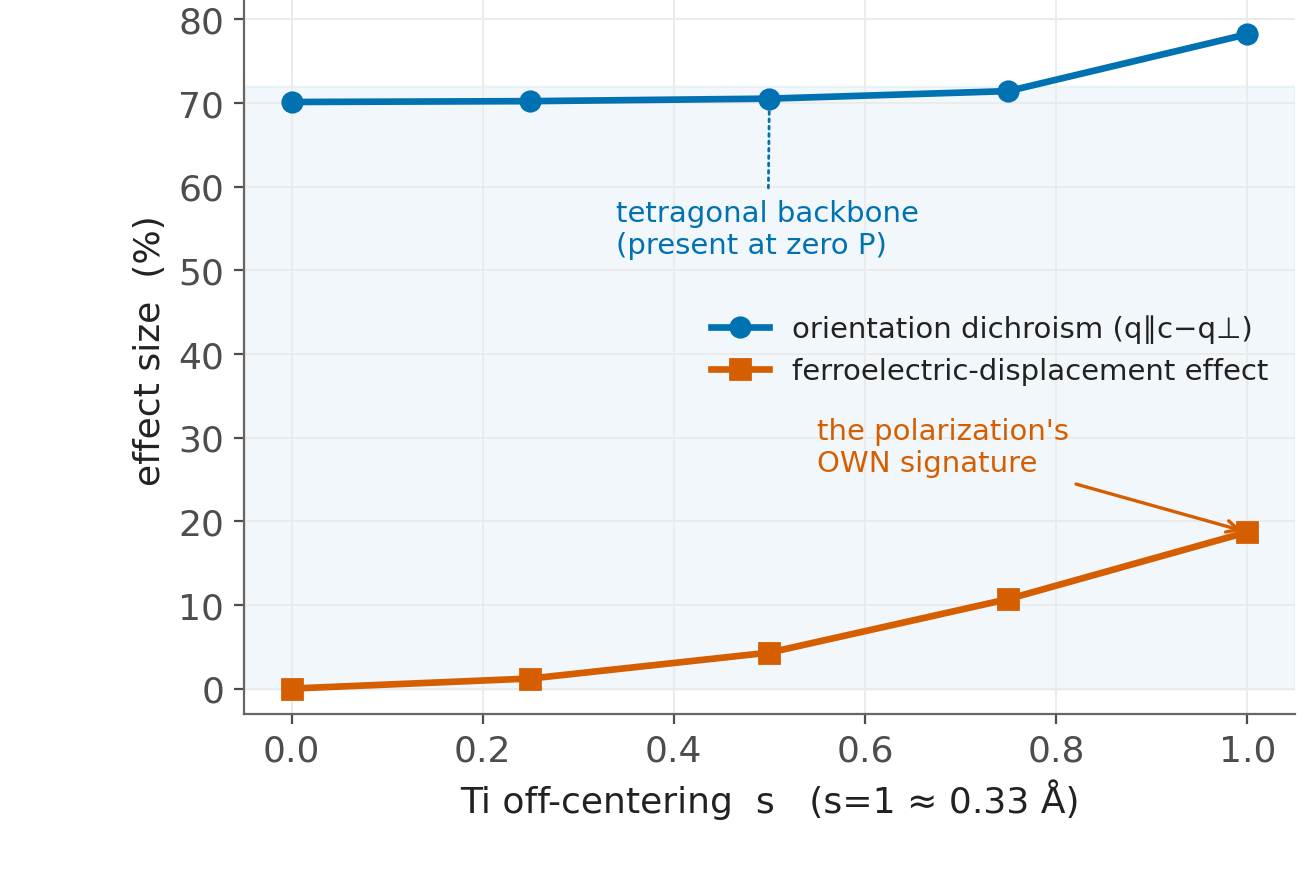
\includegraphics[width=\linewidth]{figs/eels_decomp}
  \caption{Separating strain from polarisation. Holding the lattice parameters fixed and varying
    only the internal Ti off-centring $s$, the total orientation dichroism (blue) is already
    $70\%$ at zero polarisation --- the tetragonal backbone --- while the ferroelectric
    displacement's own signature (orange) grows monotonically to $19\%$ at the experimental
    off-centring $|\mathbf{u}|\approx0.33$\,\AA.}
  \label{fig:eels-scan}
\end{figure}

% ===========================================================================
\section{Conclusions and further work}
% ===========================================================================

Fitting a reconstructed multislice-ptychographic volume as a superposition of a \emph{measured}
single-atom response recovers the oxygen sublattice of a PbTiO$_3$/SrTiO$_3$ superlattice where
the established deconvolve-then-detect workflow does not: $96\%$ bulk recall against at most
$59\%$, with the entire margin concentrated in the axially overlapped oxygen ($82\%$ against
$9$--$26\%$) that a single-orientation measurement buries under its titanium neighbour. The
advantage is not a tuning artefact --- deconvolution's limit is the axial spatial frequencies
the aperture never records --- and it comes with two things no peak detector provides: species
labels ($1.1\%$ confusion) and calibrated per-atom uncertainty.

The uncertainty machinery is, we think, the more transferable contribution. Combining a
\emph{joint} Cram\'er--Rao bound --- which recovers the twofold variance inflation that a
per-peak bound misses wherever responses overlap, and $85\%$ of atoms here have an overlapping
neighbour --- with Mondrian conformal calibration produces intervals that hold their nominal
coverage per stratum, contain no hand-tuned constant, and transfer unchanged to an independent
reconstruction at different sampling, slicing and dose, where hand-tuned error floors fail
badly (at a $68\%$ target, $69\%$ coverage against $38$--$56\%$). We would encourage the reporting of coverage rather than
of a fitted $\sigma$: the same pipeline that reads $\sigma$-calibrated at one dose reads
$38\%$ species confusion at another while its precision still reads $0.95$.

Propagated into the physics, the result is sharply two-sided. The in-plane polarisation map is
quantitative --- median error $0.007$\,\AA{} in magnitude and $0.9^\circ$ in direction, against
a $0.27$\,\AA{} signal --- while the along-beam component is not measured at all, because
differencing two $0.3$\,\AA{} depth coordinates cannot resolve a $0.07$\,\AA{} displacement.
The calibrated uncertainty establishes this without ground truth, which is precisely what such
machinery is for. First-principles core-hole DFT then shows the missing component is
spectroscopically accessible in principle: the O~K edge is $78\%$ dichroic to the polar-axis
orientation, of which a monotonic $19\%$ is the displacement's own signature rather than the
tetragonal backbone's, though the dipole limit forbids recovering the \emph{sign} and the magic
angle forbids using the $100$\,mrad ptychography aperture to do it.

Several directions follow. \emph{Method}: the one-kernel-for-all-species assumption is weakest
where it matters most, since oxygen's larger Debye--Waller factor genuinely broadens its
response under thermal scattering; in-situ vacancy-difference kernels --- the lattice
reconstructed with and without a single atom --- would supply the in-crystal oxygen matched
filter no existing kernel provides. The $5\%$ cage-composition tail of Sec.~\ref{sec:pol}, the
dominant residual error on the polarisation map, is a detection rather than a localisation
problem and needs a calibrated cage-completeness criterion; learned denoising of the volume
before fitting \citep{Wu2026} is a natural route below $10^{6}$\,e\,\AA$^{-2}$.
\emph{Physics}: the outstanding EELS cross-checks are the rotational-invariance test and the
multiplicity-weighted full O~K edge; beyond them, a faithful vortex simulation would inject a
\emph{per-atom} $\sigma(E)$ keyed to each oxygen's local polar-axis orientation, closing the
loop from the spectroscopy back onto the imaged sample. \emph{Instrument}: the clearest
experimental conclusion is a design constraint --- a combined depth-resolved-imaging and
polarisation-spectroscopy experiment cannot share one large aperture. Whether the two can be
fused into a single three-dimensional vector polarisation measurement, along the lines of
energy-filtered ptychography of the oxygen sublattice \citep{Dong2024} or momentum-selective
EELS of these very flux-closure structures \citep{Huang2026}, is the question this work leaves
open.

% ===========================================================================
\section{Reproducibility}
% ===========================================================================

All code, the input structure and the per-run parameters are in the project repository, and the
pipeline is scripted end to end: simulation (\texttt{sim/simulate\_4dstem.py}), reconstruction
(PtychoShelves \texttt{GPU\_MS}), localisation (\texttt{atomfind/run\_atomfind.py}),
polarisation (\texttt{atomfind/polarisation.py}) and the DFT staircase
(\texttt{eels/build\_cells.py}, \texttt{run\_coreloss.slurm}, \texttt{analyze\_elnes.py}), with
a unit-test suite guarding the structure generation and parsing.

\paragraph{The peer-reproducible result.} The nominated result is the localisation-with-UQ
output of Sec.~\ref{sec:pol}. A peer receives the reconstructed phase volume (a
$70\times404\times404$ array), the measured kernel, and the script; running
\texttt{run\_atomfind.py} followed by \texttt{polarisation.py} produces
\texttt{found\_atoms.csv} --- element, $(x,y,z)$ in \aa{}ngstr\"om, per-axis $95\%$ conformal
half-widths, model $\sigma$, species confidence, and a flag marking lattice-constrained
detections --- together with the conformal calibration table and the Ti--O$_6$ off-centring with
propagated uncertainty. The run takes a few minutes on one core and needs no GPU, so it is well
within the moderate resources specified; the upstream simulation and reconstruction, which are
not, are supplied pre-computed.

\paragraph{Expected values and their uncertainty.} A peer should reproduce, bit-for-bit on the
same input, $1834$ atoms with precision $0.97$; bulk recall $96/96/96\%$ for Pb/Ti/O; species
confusion $1.1\%$; in-plane RMS accuracy $0.032$\,\AA{} and depth RMS $0.37$\,\AA. The
uncertainty on each reported coordinate is the exported conformal half-width, whose validity is
the coverage statement itself: $96\%$ of true errors fall inside the $95\%$ interval, per
stratum, verified held-out on a $50/50$ split. Typical values are $0.02$\,\AA{} in-plane and
$0.5$\,\AA{} in depth, and they are strongly heteroscedastic --- up to $1.5$\,\AA{} in depth for
weak oxygen near the exit surface --- which is why the per-atom interval, not a global figure,
is the quantity to propagate. For the derived polarisation, the in-plane off-centring carries a
propagated $\sigma$ of $0.011$\,\AA{} and the along-beam component $0.237$\,\AA. The single
stochastic element is the conformal calibration split; it is seeded, and re-seeding changes the
quantiles by less than $5\%$. The known failure modes a peer should expect to see flagged are
the $28\%$ of titanium with incomplete oxygen cages and the $5\%$ with cage-composition errors,
both reported by the script rather than silently absorbed.

\begin{acknowledgments}
The relaxed PbTiO$_3$/SrTiO$_3$ supercell was provided by collaborators and is used with
their agreement; we thank them for the structure. Calculations were performed on the Warwick
Blythe cluster and the Scientific Computing RTP. TM is supported by the EPSRC HetSys Centre for
Doctoral Training (EP/S022848/1).
\end{acknowledgments}

\bibliographystyle{apsrev4-2}
\bibliography{refs}

\end{document}
